\documentclass{assignment}
\usepackage{amsmath}
\usepackage{lipsum}
\usepackage{multicol}
\usepackage{fancyhdr}
\usepackage{graphicx}
\usepackage[dvipsnames]{xcolor}
\usepackage{enumitem}

\usepackage{color,soul}
\usepackage{amsfonts}
\def\code#1{\texttt{#1}}
\usepackage{graphicx} % Required for inserting images
\graphicspath{ {./images/} }
\usepackage{booktabs}
\usepackage{xcolor}
\usepackage{mdframed}
\usepackage{bbm}
\usepackage{hyperref}
\usepackage{bookmark} % Required for enhanced bookmarks
\usepackage{cleveref}

\usepackage{algpseudocode}
\usepackage{amssymb}

\begin{document}

\assignmentTitle{assets/kth-logo.png}
{Optimization}
{Homework 1}
{SF1811}
{Lucas Frykman, Jonathan Tadesse}
{Student personal numbers: 021012-7650, 970729-4311}
{Student Emails: lfrykman@kth.se, jtadesse@kth.se}
AI level 1: Used chatgpt to parse numerical results in to latex. \\

The intent of this homework assignment is to use the simplex method for solving a linear program in standard form,

\begin{align*}
&\text{(LP)} & \min_{x \in \mathbb{R}^n} \ & c^T x \\
& & \text{subject to} \ & Ax = b, \\
& & & x \geq 0.
\end{align*}

There are Matlab functions \texttt{simplex.m} and \texttt{polyplot.m} available in Canvas to assist you.
\section*{Exercise 1}
The simplex method is an iterative method. Its aim is to find the minimum of functions of the form $z(x) = C^Tx$ with a constraint 
$Ax=b$. Here's a brief description of each step of the method.

\begin{algorithmic}
    \State \textbf{Select the initial basic index tuple}
    \State We start by selecting linearly independent columns of $A$ to form a new matrix $A_\beta$ which we call the basic matrix. 
    The basic index tuple $\beta = (\beta_1, \beta_2...\beta_m)$ are the indices of the 
    basic variables we have selected from $x$ in to $x_\beta$ corresponding to the column indices we have selected for the basic matrix. 
    After this we define our non basic matrix and non basic variable $A_\nu$ and $x_\nu$ where the non basic index tuple $\nu = (\nu_1,\nu_2...\nu_{n-m})$ are all the indices not included in $\beta$.
    Where we set $x_\nu = 0$.
    \State \textbf{Step 1:}
    \State Solve $A_{\beta}\overline{b} = b$ for $\overline{b}$. This is solvable with multiplying with $A_\beta^{-1}$. If $\bar{b}\ge 0$ this gives us the initial
    basic feasible solution for $x_\beta$. Our goal is to determine whether this solution is optimal or if we can decide on a better choice of basic variables.
    
    \State \textbf{Step 2: }
    \State Solve $A_{\beta}^T y = c_{\beta}$ for simplex multipliers $y$. (Similarly as before $c_\beta$ are the corresponding coefficients to $x_\beta$)
    
    \State \textbf{Step 3: }
    \State Calculate $r_{\nu}^T = c_{\nu}^T - y^T A_{\nu}$ to find the reduced cost with respect to the non basic variables. Observe that this value is obtained from the objective value function $z = y^Tb + (c_\nu^T - y^TA_\nu)x_\nu$
    This measures the rate the objective value function improves if our choice of non-basic variables have been increased from zero.
    
    \State \textbf{Step 4: stopping criterion}
    \If{$r_{\nu} \ge 0$}
        \State then there's no non basic variables that can perform better than the basic variables we have chosen. i.e the basic feasible solution we found in this iteration is optimal and we can stop (any further increase to  will increase the objective functin). 

        \State \Return $x_{\beta} = \overline{b}, \ x_{\nu} = 0$
    \Else
        \State \textbf{Step 5: Select entering variable}
        \State Choose index $q$ such that $r_{\nu_q} < 0$. By dantzig's rule we choose $q$ from the most negative component of $r_\nu$.
        \State Set $k = \nu_q$. We want to try to find a better BFS so we'll let $x_k = x_{\nu_q}$ be a new basic variable.
        
        \State \textbf{Step 6: }
        \State Let $x_{\nu_q} = t$ while we keep other non basic variables at $0$. The cost function will become $z = \bar{z} + r_{\nu}^Tx_\nu = \bar{z} + tr_{\nu_q}^T$ along with
        the constraint $A_\beta x_\beta + ta_k - b = 0$. We can factor out $A_\beta$ from this equation since the basic matrix is invertible 
        so we obtain that $A_\beta (x_\beta + t\bar{a}_k - \bar{b}) = x_\beta + t\bar{a}_k - \bar{b} = 0$. 

        \State so in this step we need to solve $$A_{\beta}\overline{a}_k = a_k$$
        From this we get the following result 
        $$x_\beta = \bar{b} - t \bar{a}_k$$
        If $\bar{a}_k \leq 0$ then $t$ can increase to infinity without violating feasibility and the cost $z$ will go to $-\infty$ and no optimal solution exists. But if at least one positive element exists in $\bar{a}_k$ then
        we want to calculate $t_{\max}$ to see whats the farthest we can go to decrease our cost function $z(t) = \bar{z} + tr_{\nu_q}^T$ wihtout violating feasibility. This means we can obtain a new BFS that's better than what we currently have.
        
        \State \textbf{Step 7: Ratio test (select leaving variable)}
        \State As stated in step 6, to ensure the feasibility condition $x_\beta\ge 0$ we want to know the maximum step size $t_{max}$. This tells us how much $t$ can increase before
        a variable in $x_\beta$ goes to zero. We want to remove the first basic variable that does this. Lets call the index of the leaving variable $p$.
        When calculating $t_{\max}$ we ensure $\bar{a_{ik}} >0 $ 
        and identify index $p$:
        \[
            t_{max} = \min_{i: \overline{a}_{ik} > 0} \left( \frac{\overline{b}_i}{\overline{a}_{ik}} \right) = \frac{\overline{b}_p}{\overline{a}_{pk}}
        \]
        \State \textbf{Step 8:} $\nu_q$ and $\beta_p$ change place when we update our index tuples $\beta, \nu$ then repeat from step 1
        
    \EndIf
\end{algorithmic} 

\section*{Exercise 2}
Lucas's personal number was used to get the data from \code{hw1data}. Our matrices are given by 
$$A = \begin{pmatrix}
-0.9771 & 0.9951 & 1.0000 & 0 & 0 & 0 \\
-0.0085 & 0.9947 & 0 & 1.0000 & 0 & 0 \\
1.9312 & 2.9730 & 0 & 0 & 1.0000 & 0 \\
1.9425 & -1.0206 & 0 & 0 & 0 & 1.0000
\end{pmatrix}, b = \begin{pmatrix}
1.9526 \\
2.9920 \\
14.0105 \\
6.0423
\end{pmatrix}, c = \begin{pmatrix}
-1.0324 \\
-2.9633 \\
0 \\
0 \\
0 \\
0
\end{pmatrix}$$

Where we have to solve the LP:

\begin{align*}
\min \quad & z = -1.0324\, x_1 - 2.9633 x_2 \\
\text{subject to} \quad \\
& -0.9771\, x_1 + 0.9951\, x_2 + x_3= 1.9526, \\
& -0.0085\, x_1 + 0.9947\, x_2  + x_4 = 2.9920, \\
& 1.9312\, x_1 + 2.9730\, x_2 + x_5 = 14.0105, \\
& 1.9425\, x_1 - 1.0206\, x_2 + x_6 = 6.0423, \\
& x_1, x_2, x_3, x_4, x_5, x_6 \geq 0.
\end{align*}

\begin{figure}[htbp]
    \centering
        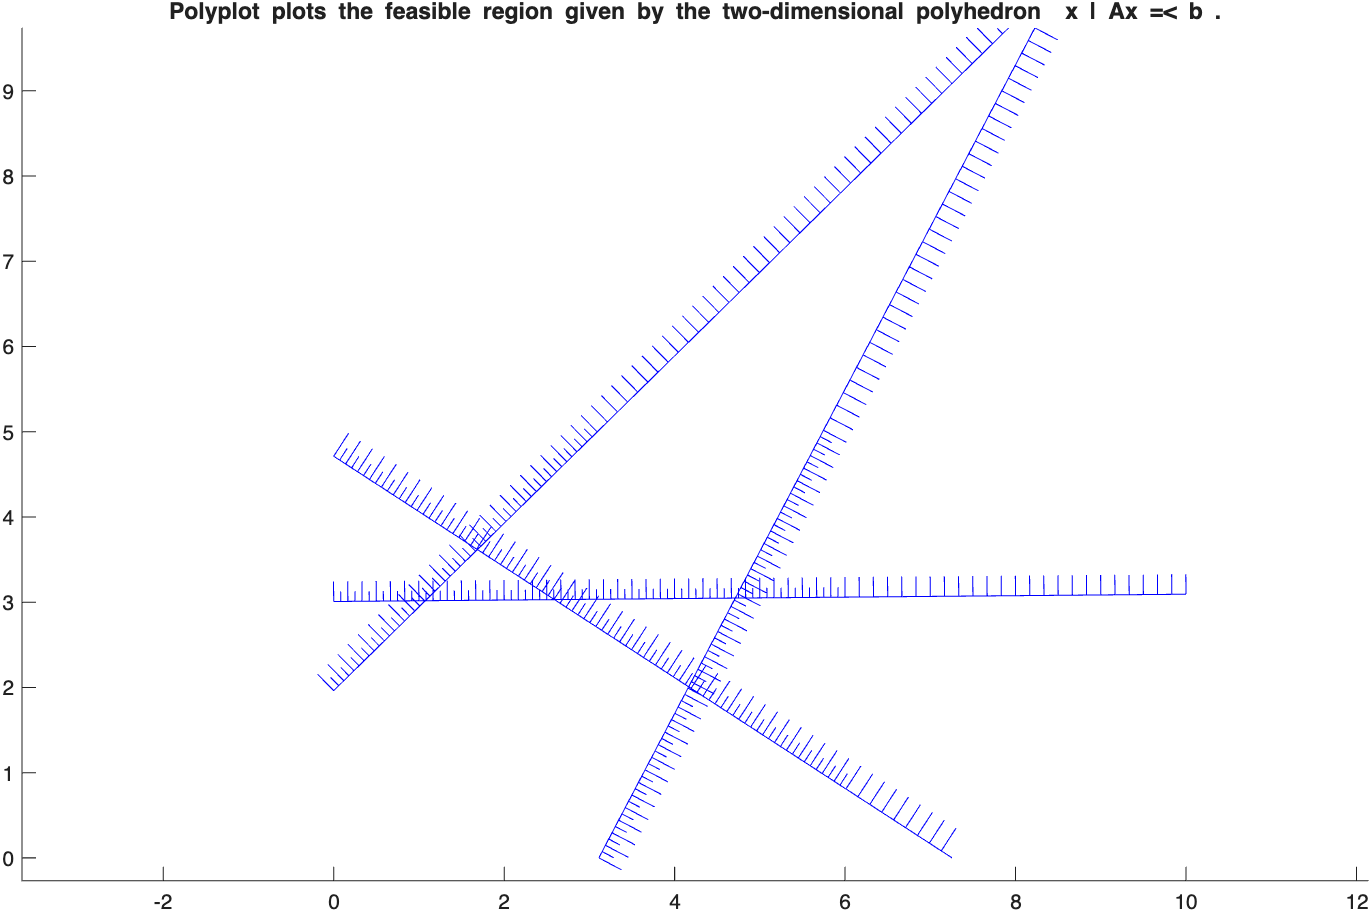
\includegraphics[width=0.8\textwidth]{assets/q2_plot.png}
        \caption{feasible region}
        \label{fig1}
\end{figure}
\newpage
\section*{Exercise 3}
 
\subsection*{\code{Iteration 1}}
\begin{algorithmic}
    \State \textbf{Step 1: Basic Solution}
    \State  We have that $A_\beta = I$ with linearly independent columns where the basic index tuple is $\beta = \begin{pmatrix} 3 & 4 & 5 & 6\end{pmatrix}$
    \State We first solve $A_{\beta}\overline{b} = b$ $\Leftrightarrow$ $ \bar{b}= \begin{pmatrix}
1.9526 \\
2.9920 \\
14.0105 \\
6.0423
\end{pmatrix}$ $\Rightarrow x^{(1)} =  \begin{pmatrix} 0 \\ 0 \\
1.9526 \\
2.9920 \\
14.0105 \\
6.0423
\end{pmatrix}$
    \State \textbf{Step 2: Simplex multipliers}
    \State Solve $A_{\beta}^T y = c_{\beta}$ for $y$ $\Leftrightarrow$ $I^Ty = y = c_\beta = \begin{pmatrix}0 \\ 0 \\ 0 \\ 0\end{pmatrix}$ 
    
    \State \textbf{Step 3: Reduced costs}
    \State Calculate $r_{\nu}^T = c_{\nu}^T - y^T A_{\nu} = c_{\nu}^T - 0^T A_\nu = c_\nu = \begin{pmatrix}-1.0324 \\ -2.9633 \end{pmatrix}$
    
    \State \textbf{Step 4: stopping criterion} 
    \State We see that $r_\nu < 0$ so the BFS isn't optimal
    \State \textbf{Step 5: Select entering variable}
    \State Choose index $q = 2$ since $r_{\nu_2} < 0$ and $r_{\nu_2} = -2.96 = \min_{\nu_i \in \nu} r_{\nu_i}$ is the most negative value of $r_\nu$. 
    \State So set $k = \nu_2$
        
    \State \textbf{Step 6: }
    \State Solve $A_{\beta}\overline{a}_k = a_k$ for $\overline{a}_k$ $\Leftrightarrow$ $I\bar{a_k} = \begin{pmatrix}0.9951 \\ 0.9947 \\ 2.9730 \\ -1.0206\end{pmatrix}$ 
    \State $\bar{a}_k$ holds positive elements so we're able to get a new BFS and continue to step 7
    \State \textbf{Step 7: Ratio test (select leaving variable)}
    \State Calculate $t_{max}$ and identify index $p$:
    $$t_{max} = \min_{i: \overline{a}_{ik} > 0} \left( \frac{\overline{b}_i}{\overline{a}_{ik}} \right) = \frac{\overline{b}_p}{\overline{a}_{pk}}$$
    We can just do a linear search over every $i$ to calculate this $$t_{max} = \min_{a_ik>0}\{ \frac{\bar{b_1}}{\bar{a_1}}, \frac{\bar{b_2}}{\bar{a_2}}, \frac{\bar{b_3}}{\bar{a_3}}, \frac{\bar{b_4}}{\bar{a_4}} \} = \min_{a_ik>0} \{ 1.9621, 3.0080, 4.7126\} = 1.9621$$.
    So the index leaving is $\beta_p = \beta_1$.
    \State Let $\nu_2 = 2$ and $\beta_1 = 3$ change place in \code{iteration 2}
\end{algorithmic} 
\subsection*{\code{Iteration 2}}
\begin{align*}
    x^{(2)} &= \begin{pmatrix} 0 \\ 1.9621 \\ 0 \\ 1.0403 \\ 8.1771 \\ 8.0447 \end{pmatrix} \\
    r_{\nu}^{(2)} &= \begin{pmatrix} -3.9421 \\ 2.9778 \end{pmatrix} \\
    y^{(2)} &= \begin{pmatrix} -2.9778 \\ 0 \\ 0 \\ 0 \end{pmatrix} \\
    \beta &= \begin{pmatrix} 2 & 4 & 5 & 6 \end{pmatrix}
\end{align*}

\subsection*{\code{Iteration 3}}
\begin{align*}
    x^{(3)} &= \begin{pmatrix} 1.0745 \\ 3.0172 \\ 0 \\ 0 \\ 2.9652 \\ 7.0343 \end{pmatrix} \\
    r_{\nu}^{(3)} &= \begin{pmatrix} 4.0716 \\ -1.0919 \end{pmatrix} \\
    y^{(3)} &= \begin{pmatrix} 1.0919 \\ -4.0716 \\ 0 \\ 0 \end{pmatrix} \\
    \beta &= \begin{pmatrix} 2 & 1 & 5 & 6 \end{pmatrix}
\end{align*}

\subsection*{\code{Iteration 4}}
\begin{align*}
    x^* &= \begin{pmatrix} 2.5900 \\ 3.0302 \\ 1.4680 \\ 0 \\ 0 \\ 4.1036 \end{pmatrix} \\
    r_{\nu}^* &= \begin{pmatrix} 1.3634 \\ 0.5406 \end{pmatrix} \\
    y^* &= \begin{pmatrix} 0 \\ -1.3634 \\ -0.5406 \\ 0 \end{pmatrix} \\
    \beta &= \begin{pmatrix} 2 & 1 & 3 & 6 \end{pmatrix}
\end{align*}
All reduced costs are $r_{\nu} \ge 0$ so we found the optimal solution.

\subsection*{\code{Optimal BFS}}
\[
x^* = \begin{pmatrix} 2.5900 \\ 3.0302 \\ 1.4680 \\ 0 \\ 0 \\ 4.1036 \end{pmatrix}
\]
\begin{figure}[htbp]
    \centering
        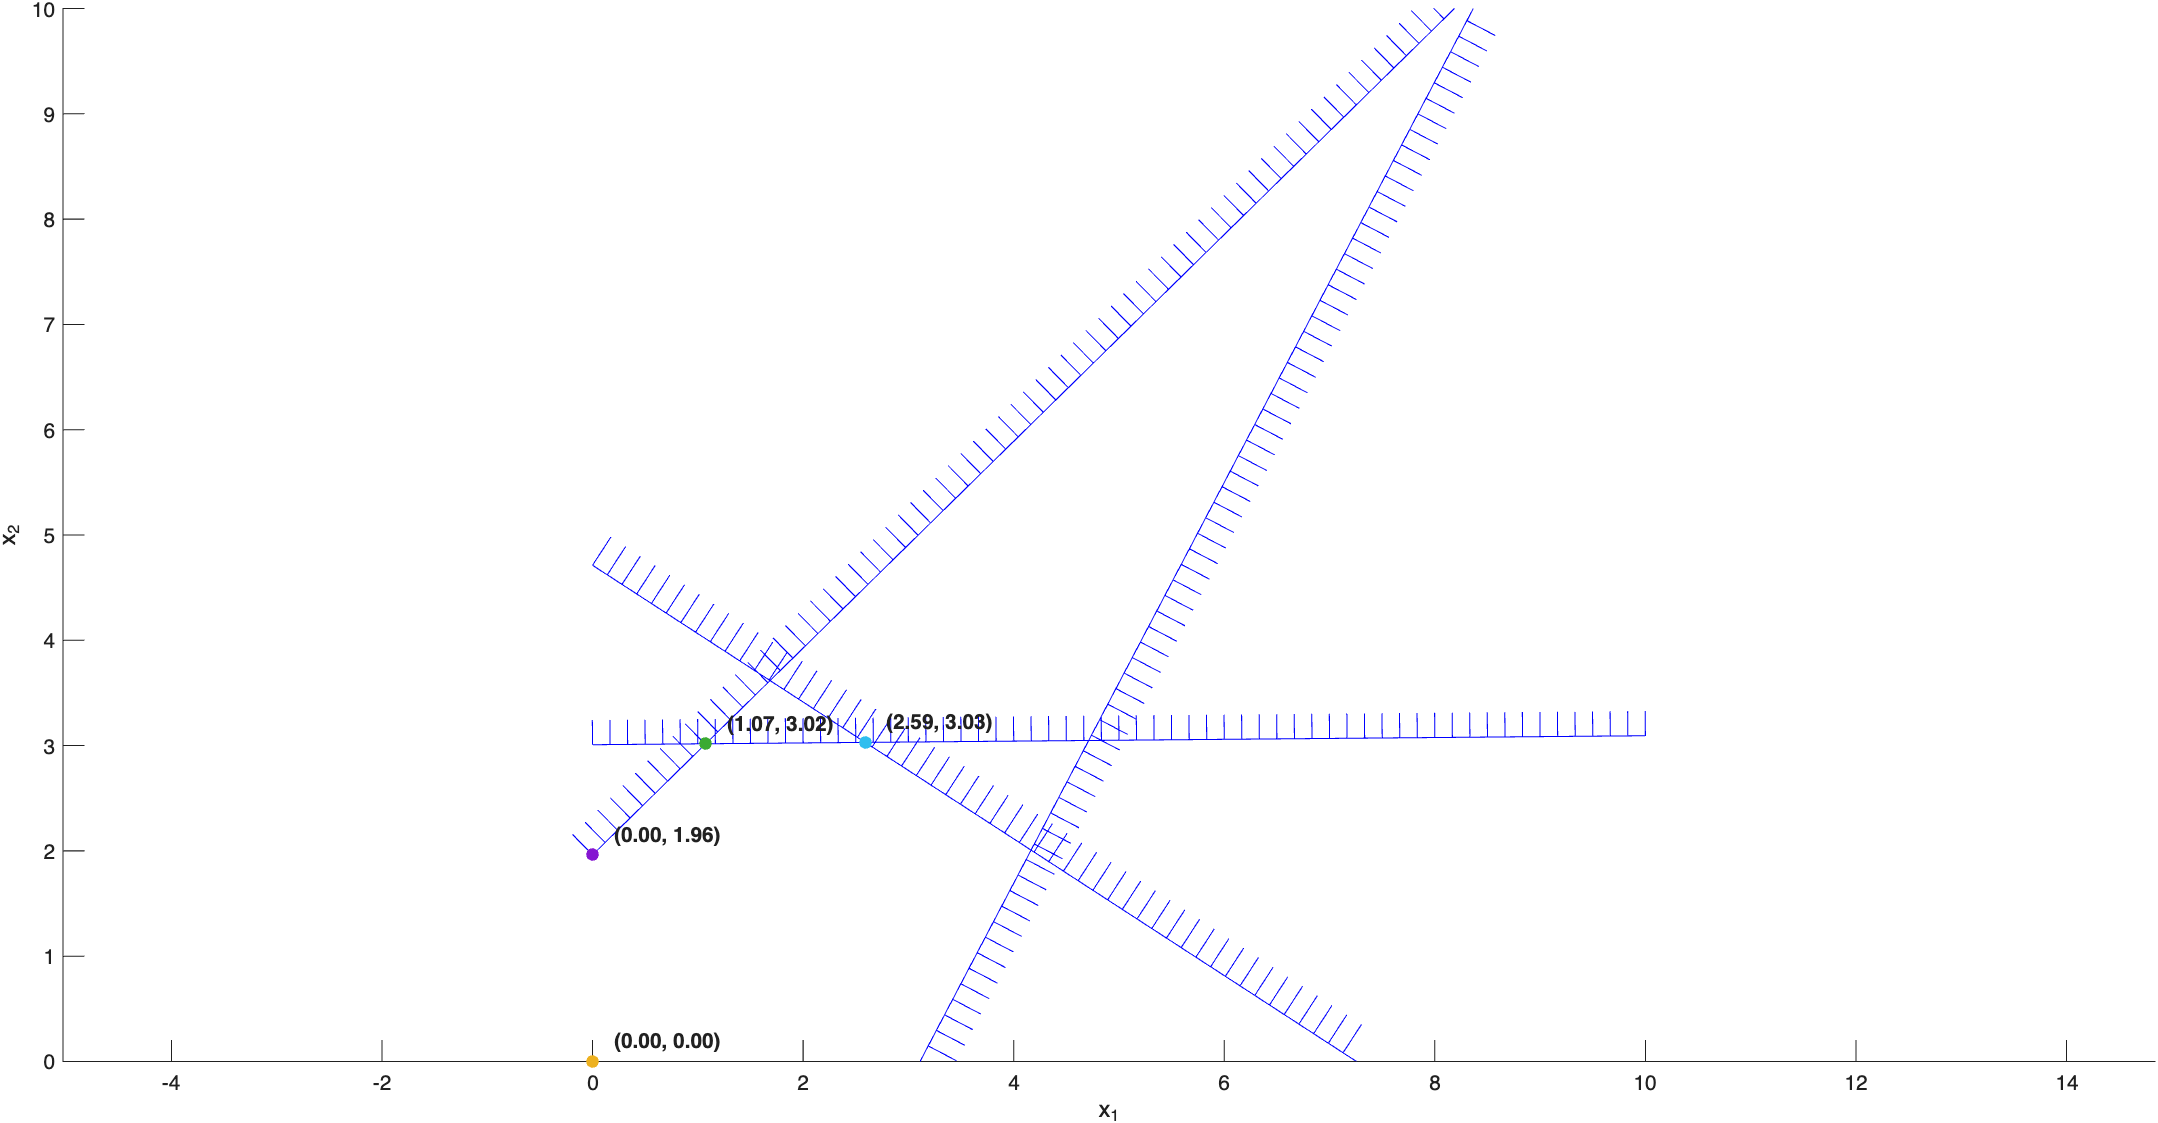
\includegraphics[width=0.8\textwidth]{assets/q3_plot.png}
        \caption{feasible region with iteration points included}
        \label{fig2}
\end{figure}
\newpage
\section*{Exercise 4}
% \subsection*{Motivation for $q = 2$ in \code{it1} in exercise 3}
% In the first iteration the reduced costs were $r_\nu = \begin{pmatrix}-1.0324 \\ -2.9633 \end{pmatrix}$. The reason why we chose $q=2$ was to get the choice of 
% basic variables for the most bang for our buck.
We'll repeat exercise 3 but with the choice of $q=1$ in \code{iteration 1}. This is still valid since $r_{\nu_1} = -1.0324 $ is also negative.
$z = \bar{z} + r_{\nu}x_\nu$. If $x_1$ becomes a basic variable it still ensures the cost decreases in the first iteration (just less than if we chose $x_2$ first). 
\subsection*{\code{Iteration 1}}
\begin{align*}
    x^{(1)} &= \begin{pmatrix} 0 \\ 0 \\ 1.9526 \\ 2.9920 \\ 14.0105 \\ 6.0423 \end{pmatrix} \\
    r_{\nu}^{(1)} &= \begin{pmatrix} -1.0324 \\ -2.9633 \end{pmatrix} \\
    y^{(1)} &= \begin{pmatrix} 0 \\ 0 \\ 0 \\ 0 \end{pmatrix} \\
    \beta &= \begin{pmatrix} 3 & 4 & 5 & 6 \end{pmatrix}
\end{align*}

\subsection*{\code{Iteration 2}}
\begin{align*}
    x^{(2)} &= \begin{pmatrix} 3.1105 \\ 0 \\ 4.9920 \\ 3.0184 \\ 8.0035 \\ 0 \end{pmatrix} \\
    r_{\nu}^{(2)} &= \begin{pmatrix} 0.5315 \\ -3.5057 \end{pmatrix} \\
    y^{(2)} &= \begin{pmatrix} 0 \\ 0 \\ 0 \\ -0.5315 \end{pmatrix} \\
    \beta &= \begin{pmatrix} 3 & 4 & 5 & 1 \end{pmatrix}
\end{align*}
\subsection*{\code{Iteration 3}}
\begin{align*}
    x^{(3)} &= \begin{pmatrix} 4.1650 \\ 2.0071 \\ 4.0251 \\ 1.0310 \\ 0 \\ 0 \end{pmatrix} \\
    r_{\nu}^{(3)} &= \begin{pmatrix} -0.3425 \\ 0.8791 \end{pmatrix} \\
    y^{(3)} &= \begin{pmatrix} 0 \\ 0 \\ -0.8791 \\ 0.3425 \end{pmatrix} \\
    \beta &= \begin{pmatrix} 3 & 4 & 2 & 1 \end{pmatrix}
\end{align*}

\subsection*{\code{Iteration 4}}
\begin{align*}
    x^* &= \begin{pmatrix} 2.5900 \\ 3.0302 \\ 1.4680 \\ 0 \\ 0 \\ 4.1036 \end{pmatrix} \\
    r_{\nu}^* &= \begin{pmatrix} 1.3634 \\ 0.5406 \end{pmatrix} \\
    y^* &= \begin{pmatrix} 0 \\ -1.3634 \\ -0.5406 \\ 0 \end{pmatrix} \\
    \beta &= \begin{pmatrix} 3 & 6 & 2 & 1 \end{pmatrix}
\end{align*}
All reduced costs are $r_{\nu} \ge 0$, optimal solution found.
\subsection*{\code{Optimal BFS}}
\[
x^* = \begin{pmatrix} 2.5900 \\ 3.0302 \\ 1.4680 \\ 0 \\ 0 \\ 4.1036 \end{pmatrix}
\]
\begin{figure}[htbp]
    \centering
        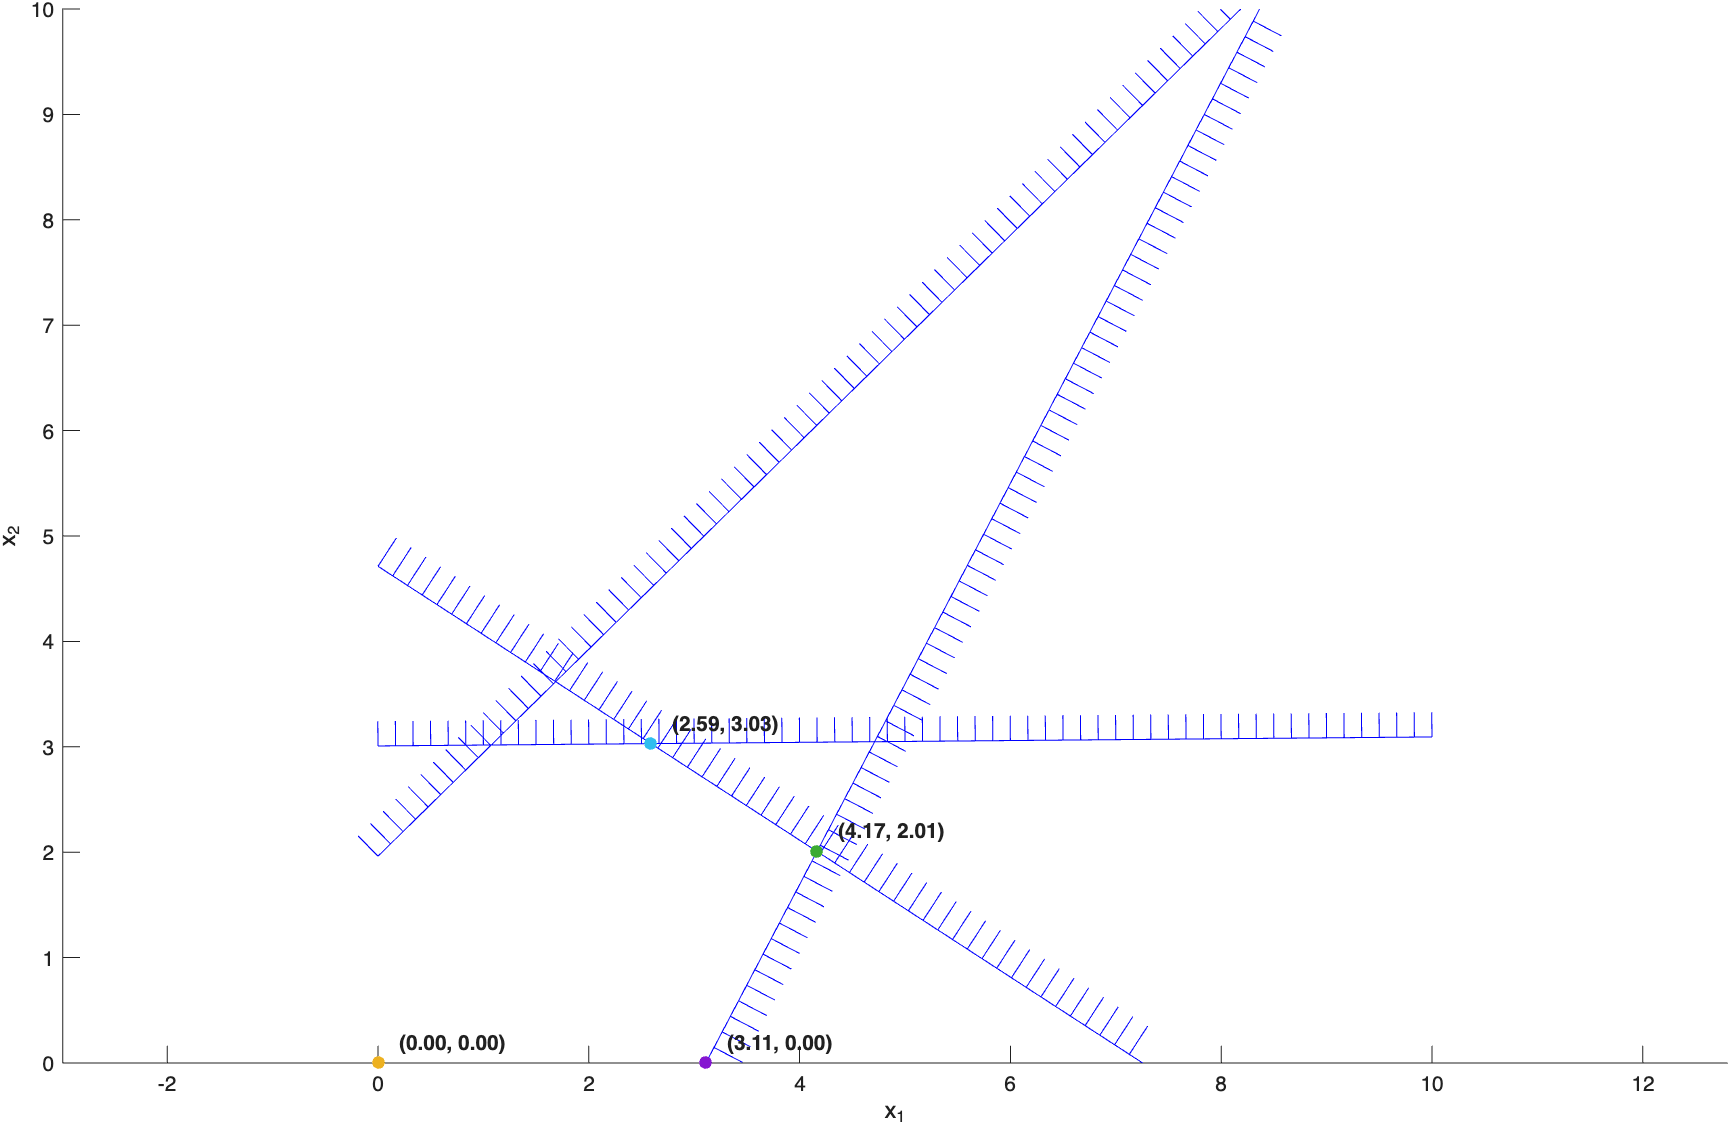
\includegraphics[width=0.8\textwidth]{assets/q4_plot.png}
        \caption{feasible region with iteration points included, but with choice of $q=1$ in \code{it1}}
        \label{fig3}
\end{figure}

\end{document}
